\documentclass[9pt]{standalone}
\usepackage{tikz}
\usetikzlibrary{matrix}
\usepackage{tikz, etoolbox}
\usetikzlibrary{arrows.meta, positioning, shapes, shapes.geometric, calc}

% Sanserif font:
\renewcommand{\familydefault}{\sfdefault}

\newcommand{\entity}[3][]{
  \node(#2)[
    entity,
    #1
  ] {
    \nodepart[font=\bfseries]{one} #2
    \nodepart{two} #3
  };
}

\tikzset{
  entity/.style = {
    draw,
    align=left,
    rectangle split,
    rectangle split parts=2,
    rectangle split ignore empty parts,
    rectangle split part align={center, left},
    minimum width=3cm,
  },
  parallellogram/.style = {
    draw,
    trapezium,
    trapezium left angle=75,
    trapezium right angle=105,
  },
  onArrow/.style = {
    fill=white,
    align=center,
  },
  has/.style = {
    -{Latex[length=3mm]},
  },
  inherits/.style = {
    -{Latex[open, length=3mm]},
  },
  bigArrow/.style = {
    -{Latex[length=5mm]},
    line width=1mm,
    font=\bfseries,
  },
  node distance=2cm and 1cm,
}

% Attempt to get a little border padding
% \usepackage[
%     left=0.20in,
%     right=0.20in,
%     top=0.20in,
%     bottom=0.20in,
% ]{geometry}


\newcommand{\dotbox}[1]{
  \begin{tikzpicture}[solid]
  #1
  \end{tikzpicture}
}

\begin{document}

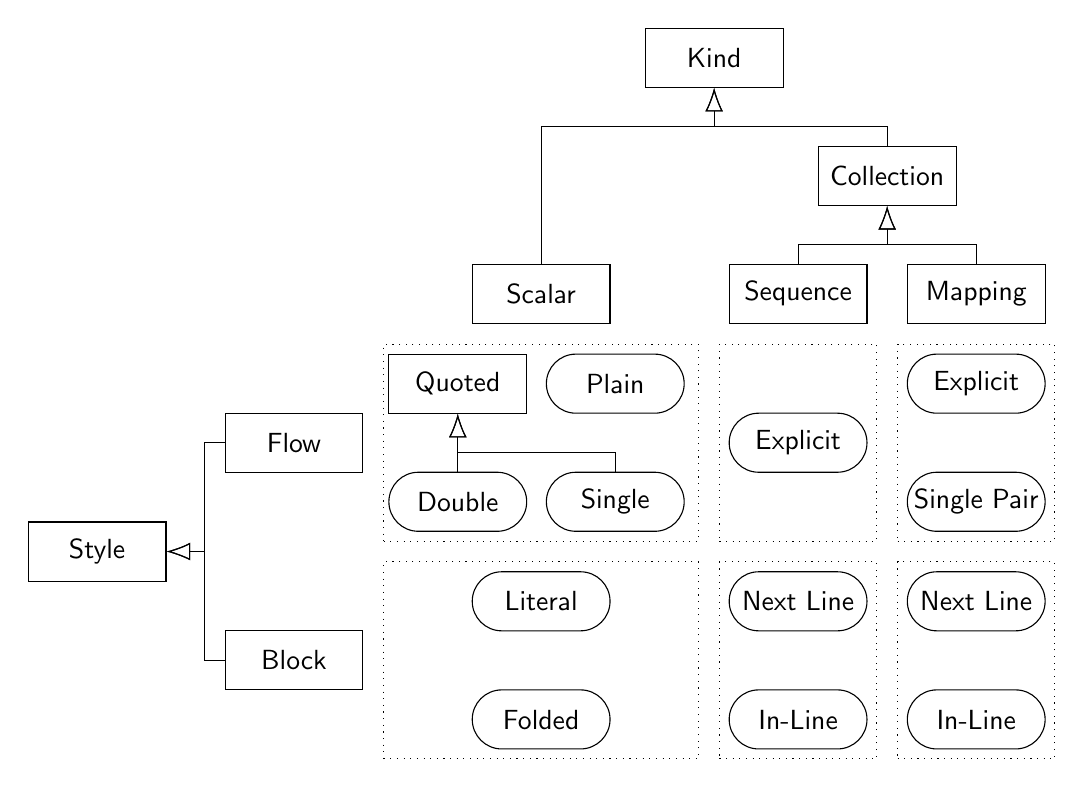
\begin{tikzpicture}[
  rect/.style = {
    draw=black,
    solid,
    rectangle,
    minimum width=1.75cm,
    minimum height=.75cm,
  },
  rounded/.style = {
    rect,
    rounded corners=0.375cm,
  },
  node distance=.25
]

\matrix(Table)[
  matrix of nodes,
  row sep={.25cm},
  column sep={.25cm},
  inner sep={0},
  nodes={
    minimum height=2.5cm,
    anchor=center,
    draw,
    dotted,
  },
  column 1/.style = {nodes={minimum width=4cm}},
] {
  \dotbox{
    \node(Double)[rounded] at (0,0) {Double};
    \node(Single)[rounded] at (2,0) {Single};
    \node(Quoted)[rect] at (0,1.5) {Quoted};
    \node[rounded] at (2,1.5) {Plain};
    \draw[inherits] (Double) -- (Quoted);
    \draw[inherits] (Single) -- ++(0,.625)  -| (Quoted);
  } &

  \dotbox{
    \node[rounded] at (0,1.5) {Explicit};
  } &

  \dotbox{
    \node[rounded] at (0,0) {Single Pair};
    \node[rounded] at (0,1.5) {Explicit};
  } \\

  \dotbox{
    \node[rounded] at (1,1.5) {Literal};
    \node[rounded] at (1,0) {Folded};
  } &

  \dotbox{
    \node[rounded] at (0,0) {In-Line};
    \node[rounded] at (0,1.5) {Next Line};
  } &

  \dotbox{
    \node[rounded] at (0,0) {In-Line};
    \node[rounded] at (0,1.5) {Next Line};
  } \\
};

\node(Block)[rect, left=of Table-2-1] {Block};
\node(Flow)[rect, left=of Table-1-1] {Flow};
\node(Style)[rect] at ($(Block)!.5!(Flow) + (-2.5,0)$) {Style};

\draw[inherits] (Flow.west) -- ++(-.25,0) |- (Style);
\draw[inherits] (Block.west) -- ++(-.25,0) |- (Style);

\node(Scalar)[rect, above=of Table-1-1] {Scalar};
\node(Sequence)[rect, above=of Table-1-2] {Sequence};
\node(Mapping)[rect, above=of Table-1-3] {Mapping};

\node(Collection)[rect] at ($ (Sequence)!.5!(Mapping) + (0,1.5) $) {Collection};
\draw[inherits] (Sequence) -- ++(0,.625) -| (Collection);
\draw[inherits] (Mapping) -- ++(0,.625) -| (Collection);

\draw let
  \p1 = (Collection),
  \p2 = ($(Scalar)!.5!(Collection)$),
  \p3 = ($(\x2,\y1) + (0,1.5)$)
in
node(Kind)[rect] at (\p3) {Kind};
\draw[inherits] (Scalar) -- ++(0,2.125) -| (Kind);
\draw[inherits] (Collection) -- ++(0,.625) -| (Kind);

\end{tikzpicture}

\end{document}
